\documentclass[dvisvgm,tikz,border=4pt]{standalone}
\usepackage{amsmath,amssymb}

\usetikzlibrary{arrows.meta,positioning,automata,shapes,shapes.misc,calc,decorations.pathmorphing,decorations.markings,angles,quotes,patterns,mindmap,matrix,knots,hobby,trees}
\tikzset{->-/.style={decoration={markings, mark=at position 0.5 with {\arrow{Stealth}}}, postaction={decorate}}}
\begin{document}
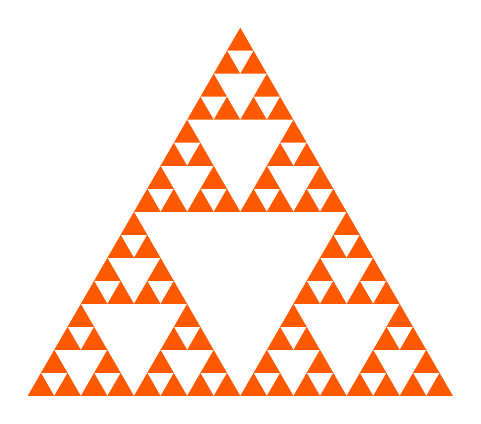
\begin{tikzpicture}[scale=0.9]
\def\tri#1#2#3#4{%
  \ifnum#4=0 \fill[orange!70!red] #1 -- #2 -- #3 -- cycle;
  \else
    \tri{#1}{($#1!0.5!#2$)}{($#1!0.5!#3$)}{\numexpr#4-1\relax}
    \tri{($#1!0.5!#2$)}{#2}{($#2!0.5!#3$)}{\numexpr#4-1\relax}
    \tri{($#1!0.5!#3$)}{($#2!0.5!#3$)}{#3}{\numexpr#4-1\relax}
  \fi}
\tri{(0,0)}{(6,0)}{(3,5.196)}{4}
\end{tikzpicture}
\end{document}
